\section{Introduction}
\label{sec:intro}

Caches play an important role in modern microprocessors by mitigating the
bandwidth and latency limitations of accessing main memory. Future computer
systems also face power and energy scaling challenges and caches play an
important role in reducing the memory system energy. Hence, it is important to
improve the cache utilization at all levels of the memory hierarchy. 

Cache/memory compression is a technique used to increase on-chip cache capacity
and to decrease on-chip and off-chip bandwidth usage. It is based on the
observation that there is significant redundancy and replication in data stored
either in main memory or in caches which enables storage of data in a more
efficient compressed format. It can be applied using software, hardware or a
combination of both. A key benefit of compression is the increased effective
storage capacity but it also helps reduce off-chip bandwidth and memory traffic
by sending and receiving data in the compressed format. Compression algorithms
like Lempel-Ziv~\cite{lemp-ziv} and Base-Delta-Immediate Compression~\cite{bdi} when implemented in
hardware could potentially improve code performance by reducing the number of
long latency accesses to the main memory. There are also potentially significant
power savings by keeping more data in the cache. 

However, there are a few challenges that need to be addressed in order to
effectively exploit these mechanisms. Compression algorithms like
Base-Delta-Immediate Compression leverage patterns, redundancy and similarity in
the data sets. In other words, these algorithms do not work on data with high
dynamic ranges. Another limitation is that the compressibility also depends on
the layout of data in memory. Different data types usually do not compress well
together because the difference in the range of values tend to be very
different. For example. chars, ints, pointers, floats etc. can be expected to
have very different byte sequences in memory. Hardware-based compression is
often effected at the granularity of a cache line. To increase the potential
compression ratio it is desirable that all the data stored in a single cache
line have low dynamic ranges - and, as explained above, similar data types. 

The aim of this project is  to explore compression-conscious data placement
optimizations using the compiler to place data fields with small dynamic ranges
spatially close together in memory. The benefits of these optimizations could
potentially be not only improved compressibility of data in caches and memory
but also simpler logic in the compression hardware. The data layout in memory
usually depends on the choice of data structures used by the programmer. Arrays
of structs are very commonly used to store data sets with disparate fields. A
struct can have many fields with different data types which are placed
contiguously in memory. In these cases the cache line storing the data may not
be very compressible. Also, because of alignment requirements, there is possibly
a lot of wastage of space in the cache line when these data structures are
padded.  

In this project, we evaluate {\em data splitting}  as a compiler technique to
improve the compressibility of data stored in memory. We, however, limit the
scope of our evaluation to cache compression although this compiler optimization
could also potentially aid memory compression. Data splitting involves splitting
a structure with multiple fields into arrays comprising the different fields in
the original data structure. By placing all the data from the same field across
all nodes or structures in a single array.

\begin{figure}[htb]
\centering
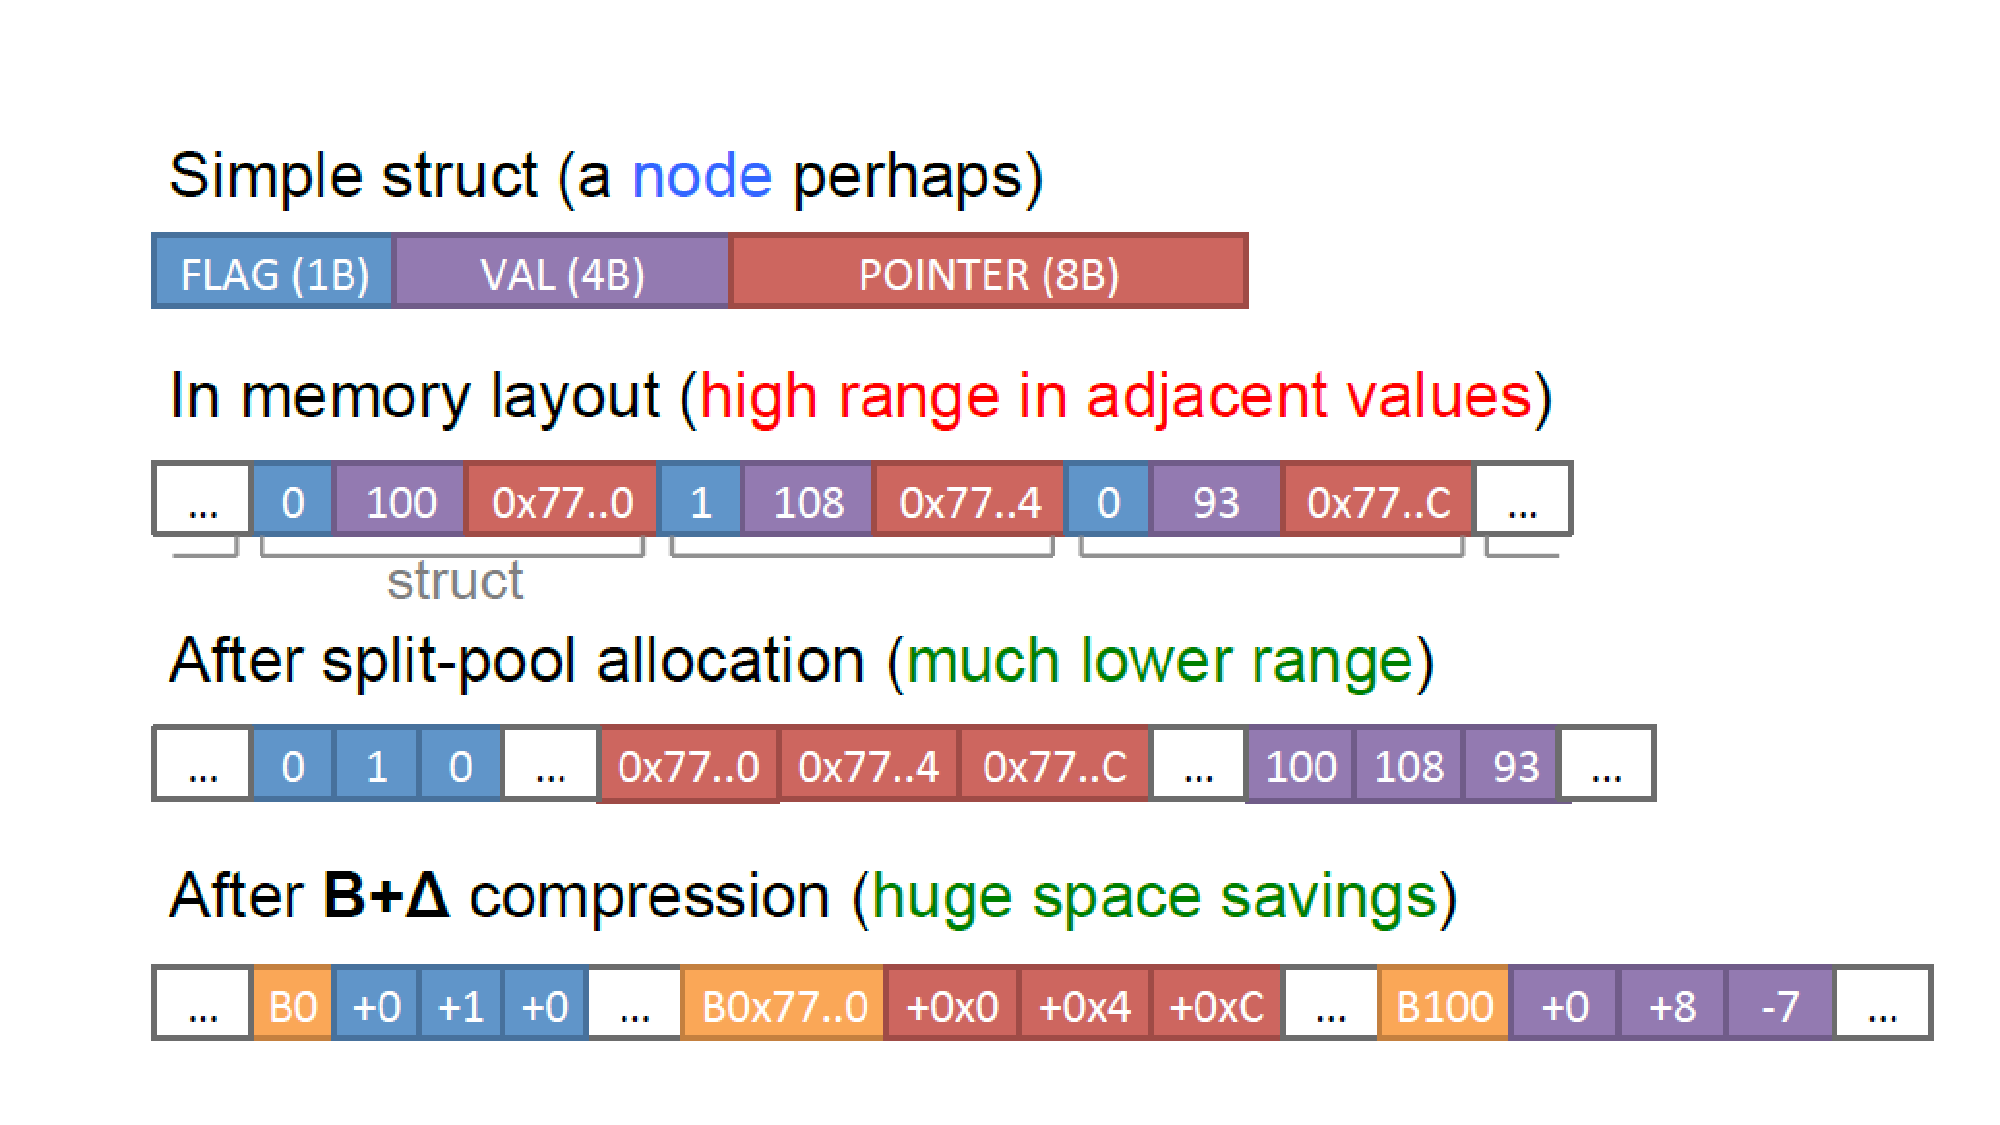
\includegraphics[trim=0mm 0mm 0mm 0mm,clip,width=1\linewidth]{figs/pic1.pdf}
\caption{Benefits of data splitting and cache compression.}
\label{fig:benefit}
\end{figure}

There are multiple ways in which splitting data structures may improve
performance. If the program only accesses a few fields frequently at any given
time, placing these hot fields together in memory can actually improve cache
locality and lead to better utilization of the cache and effectively reduces the
working set size, reduces the memory traffic, reduces the number of capacity
misses and does not pollute the cache. Splitting data also creates data streams
that can be prefetched by hardware prefetchers. Most hardware prefetchers can
prefetch from multiple data streams simultaneously and by making the access
pattern more regular, the prefetch accuracy could be potentially higher~\cite{mpads}.
Here, we implement and evaluate the benefits of data splitting in generating
data layouts that are more amenable to data compression.

Section details all aspects of our optimization implementation in LLVM. Section
describes the evaluation details including our simulation infrastructure and
testing benchmark.  Section contains a detailed evaluation of our performance
results and experiments.  We discuss related work and future work in
Section~\ref{sec:rel}
and Section~\ref{sec:fut} and conclude in Section~\ref{sec:conc}
